\documentclass[12pt,a4paper]{article}

\usepackage{fontspec}
\usepackage{polyglossia}
\usepackage[left=3cm,top=2cm,right=1cm,bottom=2cm,nohead]{geometry}
\usepackage{setspace}
\usepackage{listings}
\usepackage{graphicx}
\usepackage{color}
\usepackage{float}
\usepackage{caption}
\usepackage{subcaption}
\usepackage{courier}
\usepackage{bold-extra}
\usepackage{fix-cm}
\usepackage{alltt}
\usepackage{indentfirst}
\usepackage{amsmath, amsthm, amssymb}
\usepackage{url}

\defaultfontfeatures{Mapping=tex-text}

\setmainfont
    [ Path           = fonts/ ,
      UprightFont    = *-Regular,
      BoldFont       = *-Bold ,
      ItalicFont     = *-Italic ,
      BoldItalicFont = *-BoldItalic]
    {LiberationSerif}
\setsansfont
    [ Path           = fonts/ ,
      UprightFont    = *-Regular,
      BoldFont       = *-Bold ,
      ItalicFont     = *-Italic ,
      BoldItalicFont = *-BoldItalic]
    {LiberationSans}
\setmonofont
    [ Path           = fonts/ ,
      UprightFont    = *-Regular,
      BoldFont       = *-Bold ,
      ItalicFont     = *-Italic ,
      BoldItalicFont = *-BoldItalic]
    {LiberationMono}

\setmainlanguage{ukrainian}
\setotherlanguage{english}



\graphicspath{{./images/}}

\setstretch{1.1}

\definecolor{javared}{rgb}{0.6,0,0}
\lstdefinelanguage{Smalltalk}{ 
  morekeywords={true,false,self,super,nil}, 
  sensitive=true, 
  morecomment=[s]{"}{"}, 
  morestring=[d]', 
} 
 
\lstset{
	basicstyle=\footnotesize\ttfamily,
	tabsize=3,
	showspaces=false,
	stringstyle=\color{javared},
	showstringspaces=false,
	xleftmargin=	.6cm
}

\begin{document}
\pretolerance=-1
\tolerance=2300

\pagenumbering{arabic}
\pagestyle{empty}
\setlength{\parindent}{1.5cm}
\fontsize{14pt}{6mm}\selectfont

\begin{center}
  Міністерство освіти і науки, молоді та спорту України
  
  Львівський національний університет імені Івана Франка

  Факультет прикладної математики та інформатики
\end{center}

\vspace{1cm}

\begin{flushright}
  Кафедра програмування
\end{flushright}

\vspace{4cm}

\begin{center}
  {\bfseries\Large Розширення функціональності моделі FAMIX для побудови абстрактних дерев коду Java-- та Smalltalk--програм}
\end{center}

\vspace{2cm}

\begin{small}
\begin{flushleft}\leftskip8.5cm
  Магістерська робота студента групи ПМІ-51м\\
  Тимчука Ю.А.\linebreak
  
  Науковий керівник:\\
  доц. Рикалюк Р.Є.
\end{flushleft}
\end{small}

\vspace{5cm}

\begin{center}
  Львів - 2013 
\end{center}

\clearpage



\setstretch{1.5}
\fontsize{14pt}{6mm}\selectfont

\tableofcontents
\clearpage
\pagestyle{plain}
\section{Вступ}

Мета--моделювання було створено, щоб дозволити розглядати програми на більш високому рівні абстракції, ніж це дозволяють поточні мови програмування. Основна ідея полягає в тому, що хтось визначає високорівневу модель рішення, описує, як перетворити це рішення в програму для даної мови, а потім автоматично генерує вихідний код. В ідеалі такий же підхід дозволяє взяти існуючу програму, автоматично отримати абстрактну модель з неї, вручну розширити або поліпшити модель і згенерувати нову програму, можливо, на новій мові програмування (round-trip engineering). Такий підхід був би дуже цікавим для організацій, що мають програми написані на старих технологіях (наприклад, Cobol) і хочуть перенести їх на більш сучасні (наприклад, Java). Команда RMoD вже має інструменти, які можуть приймати програми (написані на C, Java, Smalltalk, і т.д.) в якості вхідних даних і продукувати з них моделі.

Тим не менш, чорт сидить в деталях, в даному випадку, для зворотньої розробки існуючої програми, щоб мати можливість відновити її потім, треба тримати багато деталей по цю програму. Ця потреба, звичайно, не сумісна з ідеєю абстрагування моделі цієї програми. Тому потрібно, бути в змозі створити абстрактну модель програми, але, в той же час, створити дуже детальну модель тієї ж програми і таким чином, мати можливість працювати на двох рівнях абстракції одночасно.

Як приклад можна розглянути дві об'єктно-орієнтовані мови програмування: Java та Smalltalk. Обидві мають подібну структуру: простори імен, класи, поля та методи класів. Але у мові Smalltalk відсутні інструкції галуження та циклу, які, безперечно, відіграють важливу роль в Java коді. З другого боку код Java не має нічого аналогічного до блоків у мові Smalltalk, які дозволяють реалізовувати галуження та цикли за допомогою методів.

Метою цієї магістерської роботи є розширення вже існуючої мета--моделі FAMIX шляхом додавання до неї компонент абстрактних синтаксичних дерев мов програмування Java та Smalltalk.

\subsection{Перспективи використання}
Абстрактні синтаксичні дерева зазвичай використовуються при компіляції, але дана мета--модель спрямована на візуалізацію вихідного коду, і таким чином надання інструментів для кращого розуміння та маніпуляції над ним.

Маючи в своєму розпорядженні універсальне дерево, яке можна буде розширювати для різних мов, слідуючи простим правилам, можна розробляти алгоритми, які, відповідно, будуть працювати для всіх розширень дерева. Таким чином можна буде зробити інстумент для моделювання прогам написаних практично будь-якій мові програмування вез значних затрат ресурсів. Серед можливих алгоритмів можна виділити:

\textbf{Symbol resolution}: сутність змінної в абстрактних синтаксичних деревах несе лише інформацію про назву змінної, цього доволі мало для аналізу вихідного коду. Одинаковий ідентифікатор може зустрічатись в різних місцях програми, але відноситись до різних змінних.

\textbf{Інтерфейс взаємодії}: модель являє собою лише пов'язані між собою сутності з параметрами. Для полегшення роботи з моделлю потрібно розробити первний інтерфейс взаємоді, наприклад: графічну оболонку, мову запитів.

\textbf{Перевірка правил}: маючи модель вихідного коду можна реалізувати перевірку деякий правил, щоб виявити „поганий“ код, як наприклад: \lstinline$if (false) {...}$.

\textbf{Генерація коду з моделі}: якщо можна було б генерувати код програми з наявної моделі, то це б можна було використати для рефакторинку програм шляхом взаємодії з графом моделі у графічному інтерфейсі. Можливо аналогічний підхід можна було б завтосовувати для побудови програм.

\textbf{Перетворення між мовами}: маючи в наявності реалізацію вищезазначеного функціоналу можна було б розробити перетворення коду з однієї мови в іншу. Звичайно, неможливо написати алгоритм, який буде генерувати ідеальний конд на новій мові програмування, але навіть можливість згрубша перевести програмне забезпечення, яке складається з мільйонів радків коду було б корисною можливістю.

\clearpage

\section{Moose}

В рамках цієї роботи використовується платформа з відкритим кодом Moose\cite{moose}, яка призначенна для аналізу систем програмного забезпечення та даних в цілому. Ця платформа написана на мові програмування Smalltalk та інтегрується безпосередньо в середовище Pharo. Ядро Moose надає можливість збереження та взаємодії із сутномсями моделей. Для цього використовуються три базові класи: \emph{Entity}, \emph{Group} та \emph{Model}.

Клас Entity(сутність) є базовим представленням сутності у моделі. Тому передбачено, що конкретні сутності специфічних мета--моделей будуть наслідуватись саме від цього класу. Entity надає два загальні сервіси. Перший - це зв'язок з моделлю до якої належить дана сутність. Це веде до циклічної залежності між моделлю та сутністю, але з одного боку така реалізація нікому не заважає, а з другого - дозволяє легко формувати запити, які потребують більшу кількість інформації аніж дана сутність може надати. Другою важливою особливістю Entity є механізм управління станами і розширенням, який досягається за рахунок ієрархії EntityState. Ця їєрархія надає словник, в якому можна зберігати дані про сутність, зокрема кешувати дані отримані підчас виконання запитів.

Клас Group(група) - це сутність, яка відображає колекцію сутностей. Наприклад, у нас може бути група сутностей класів, чи група сутностей методів. Групи є важливою абстракцією, особливо для виконання запитів та користувацького інтерфейсу.

Клас Model(модель) по своїй суті є сукупністю сутностей та їх внутрішніх зв'язків для вибраної системи. Це спеціальний підвид групи.

Moose використовує сім'ю мета-моделей під назвою FAMIX. Вони можуть бути використані для представлення моделей пов'язаних з різними аспектами систем програмного забезпечення. Ці мета-моделі зазвичай спрамовані на полегшення аналізу,  і надають багатий API для здійснення запитів та навігації. Ядро FAMIX складається з узагальненої мета-моделі, яка може відобразити багато об'єктно--орієнтованих та процедурних мов. 

\clearpage

\section{Основні ідеї FAST}

FAST являє собою інфрастуктуру з трьох частин: модель, завантажувач та додатки.

Остовна ідея \emph{моделі} --- це визначення структури, яку можна буде використовувати для репрезентації коду у вигляді абстрактного синтаксичного дерева. Ця модель слідує основним принципам FAMIX. Тобто створюється ядро моделі, яке визначає структуру одинакову для всіх мов програмування. Тоді для кожної мови програмування створюється розширення, яке додає свої специфічні ланки.

Щоб ця система була актуальною для використання, необхідно мати можливість генерувати молелі безпосередньо з вихідного коду методу. Для цього використовується \emph{завантажувач}. Він слідує попередній стратегії, втім ядро завантажувача доволі мале, так як кожна мова вимагає окремого підходу для завантаження.

\emph{Додатки} мають на меті опрацювання моделі. Тобто алгоритми для визначення метрик, або відвідувач для траверсу моделі. Осномна ідея додатків полягає в тому, що вони не мають сильно відрізнятись для кожної мови (крім відвідувача).

\subsection{Модель}

Абстрактне синтаксичне дерево зазвичай використовується компілятором як основа для генерування байт--коду. В нашому ж випадку модель абстрактного ситтаксичоно дерева має містити якомога більше кількітьсь інформації для того, щоб дозволити нам проводити аналіз різного типу на її основі. З цією ж метою мета--модель, яку ми розробляємо буде мкасимально зв'язаною з існуючою мета--моделлю.

\textbf{Вираз (Expression)} --- це частина коду, яка має певне значення. Це може бути літерал, змінна, виклик функції (чи методу). Вираз може бути присвоїним змінній чи переданим як аргумент.

Виконавче тіло методу складається з \textbf{речень (Statement)}. Кожне речення являє собою повноцінну виконавчу ланку. Яскравими прикладами речень є інстукція галуження \lstinline$if$, інструкції циклів, або ж речення, яке вказує на повернення з методу. Також часто зустрічаються речення які просто містять вираз, наприклад:
\begin{lstlisting}[language=Java]
System.out.printl("Hello world");
\end{lstlisting}

Часто важко побачити різницю між виразами та реченнями. Перш за все збивають речення які не містять нічого іншого крім виразу. Наприклад
\begin{lstlisting}[language=Smalltalk]
5 factorial
\end{lstlisting}
це вираз. Ми його можем передати як параметер повідомлення або ж відправити повідомлення йому самому:
\begin{lstlisting}[language=Smalltalk]
'Factorial of 5: ', 5 factorial asString
\end{lstlisting}
Наступний приклад є реченням:
\begin{lstlisting}[language=Smalltalk]
5 factorial.
\end{lstlisting}
В смолтоці крапки використовуються як розділювачі для реченнь. Даний приклад доволі концептуальний, але головне його покликання --- показати, що речення --- це сутності на найвищому рівні виконавчого коду. І не зважаючи на те, що деякі речення можуть складатись з лише одного виразу --- це всеодно речення і вони є абсолютно відмінними від сутностей.

З другого боку різні мови мають різні правила. Наприклад в смолтоку присвоєння є виразом, тому ми можемо написати:
\begin{lstlisting}[language=Smalltalk]
list add: x := 5 factorial
\end{lstlisting}
цей код обчислить $5!$ присвоїть його змінній $x$ а потім додасть ці значення до списку. В мові програмування \emph{Basic} присвоєння є реченням, це також часто призводить до непорозумінь між термінами.

Давайте розглянемо приклад:
\begin{lstlisting}[language=Smalltalk]
middleOf: a and: b
    | sum |
    sum := a + b.
    ^ sum / 2
\end{lstlisting}
Перші два рядки відносяться до оголошення методу та тимчасових змінних, тому зараз можемо їх опустити. У даному прикладі присутні два \emph{речення}:
\begin{enumerate}
	\item \lstinline$sum := a + b$
	\item \lstinline$^ sum / 2$
\end{enumerate}
А також близько пів--дюжини \emph{виразів}: \lstinline$sum := a + b$, \lstinline$sum$, \lstinline$a + b$, \lstinline$a$, \lstinline$b$, \lstinline$sum / 2$, \lstinline$2$.

Не зважаючи на те, що я розробляю окремі моделі для кожної з мов, за основу було вибрано ідею, яка передбачає стандартні правила для всіх моделей. Цю ідею можна сформулювати наступним чином:
\begin{enumerate}
  \item Виконавча частина функції(методу) є послідовністю речень.
  \item Речення може містити вирази або ж виконавчі блоки.
  \item Виразом є сутність, яка має значення.
\end{enumerate}
Тому в наступних моделях у нас будуть присутні базові типи \emph{речення} та \emph{вираз}, при чому без будь-яких безпосередніх зв'язків. Звичайно, в їхні наслідники можуть залежати одне від одного, але на найвищому рівні ми таких обмежень не накладаєм.

В якості узагальнення всіх посилання на сутності задопомогою їхнього ім'я використаємо \textbf{іменовану сутність (Named Entity)}. Прикладом може бути використання будь-якої змінної для присвоєння їй значення чи використання значення на яке вона вказує, або ж назва класу метод якого буде викликатись. Ця сутність буде зв'язана з іменованою сутністю FAMIX, яка в свою чергу може бути локальною чи глобальною змінною, параметром, змінною класу, неявною змінною, або ж класом.

\textbf{Cутність з поведінкою (Behavioural Entity)} - це сутність, яка має в собі певний код, який виконується --- поведінку. Наприклад методи, функції, замикання та лямбда--функції є такими сутностями. Ця сутність має набір \emph{речень}, а також два набори \emph{іменованих сутностей} в якості параметрів та локальних змінних. \emph{Cутність з поведінкою} буде слугувати коренем для нашого дерева. Логічним розширенням буде \textbf{іменована сутність з поведінкою (Named Behavioural Entity)}, так як методи та функції мають ім'я чи селектор за яким їх можна ідентифікувати. \emph{Іменована сутність з поведінкою} в свою чергу буде зв'язана з іменованою сутністю FAMIX, так як остання передбачає в собі наявність селектора.

\begin{figure}[h]
  \centering
    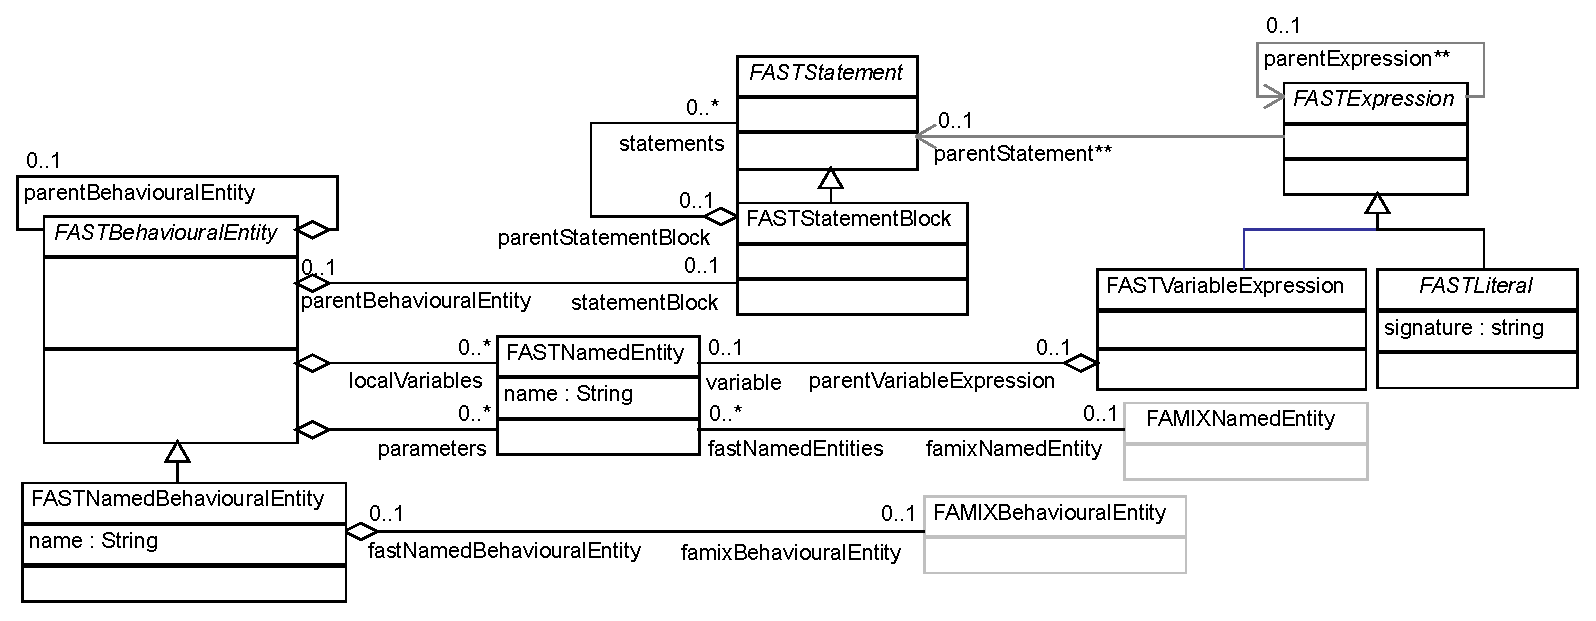
\includegraphics[width=0.95\textwidth]{GeneralASTClassDiagram}
  \caption{Базова структура FAST\label{genFast}}
\end{figure}

На рис.~\ref{genFast} показано діаграму основи моделі. Префікс \textbf{FAST} - це назва моделі, означає він Famix AST.

\subsubsection{Квазі--загальні ланки}

Посеред мов програмування присутні подібні конструкції, які можуть зустрічатись не у всіх мовах, або ж мати невелику різницю. Наприклад, це речення, яке повертає значення з методу. З дного боку --- це дуже поширена конструкція, яка просто незамінна у багатьох мовах програмування. З другого --- синтакс у Smalltalk та Java дещо інший, ланка повернення для обох мов має себе поводити дещо інакше. Також, якщо подивитись на функціональну мову програмування SML, то в неї немає такого поняття, як речення, що поветають значення, адже кожне речення має цю поведінку. Якщо ж вважати, що кожне речення SML є ланкою повернення, то звідси випливає, що в таких мовах немає речення, яке містить просто вираз. На даний момент прийнято рішення в кожній мові визначати свої ланки. Наприклад в поточній реалізації мають місце ланки FASTSmalltalkReturnStatement та FASTJavaReturnStatement.

\clearpage

\section{Мета--модель абстрактного дерева Smalltalk}

Абстрактне синтаксичне дерево смолтоку вражає. Не зважаючи на те, що у FAST--варіанті смолтоку присутні „зайві“ ланки, які призначені для сумісності з іншими мовами, це дерево складається лише з двадцяти семи ланок. Навіть синтакс смолтоку містить в три рази менше граматичних елементів аніж синтакс джава\cite{meet-grammars}. Робота з смолтоком була першою ціллю цього проекту, так як абстрактне синтаксичне дерево достатньо мале і просте, для того, щоб його змоделювати повною мірою. В той же час смолток якляє собою повноцінну мову, на якій можна реалізувати рішення основних проблем, які виникають при еволюції програмного забезпечення.

\subsection{Структура моделі}

Діаграма класів моделі абстрактного синтаксичного дерева смолтоку рис.~\ref{smtFast}.

\begin{figure}[h]
  \centering
    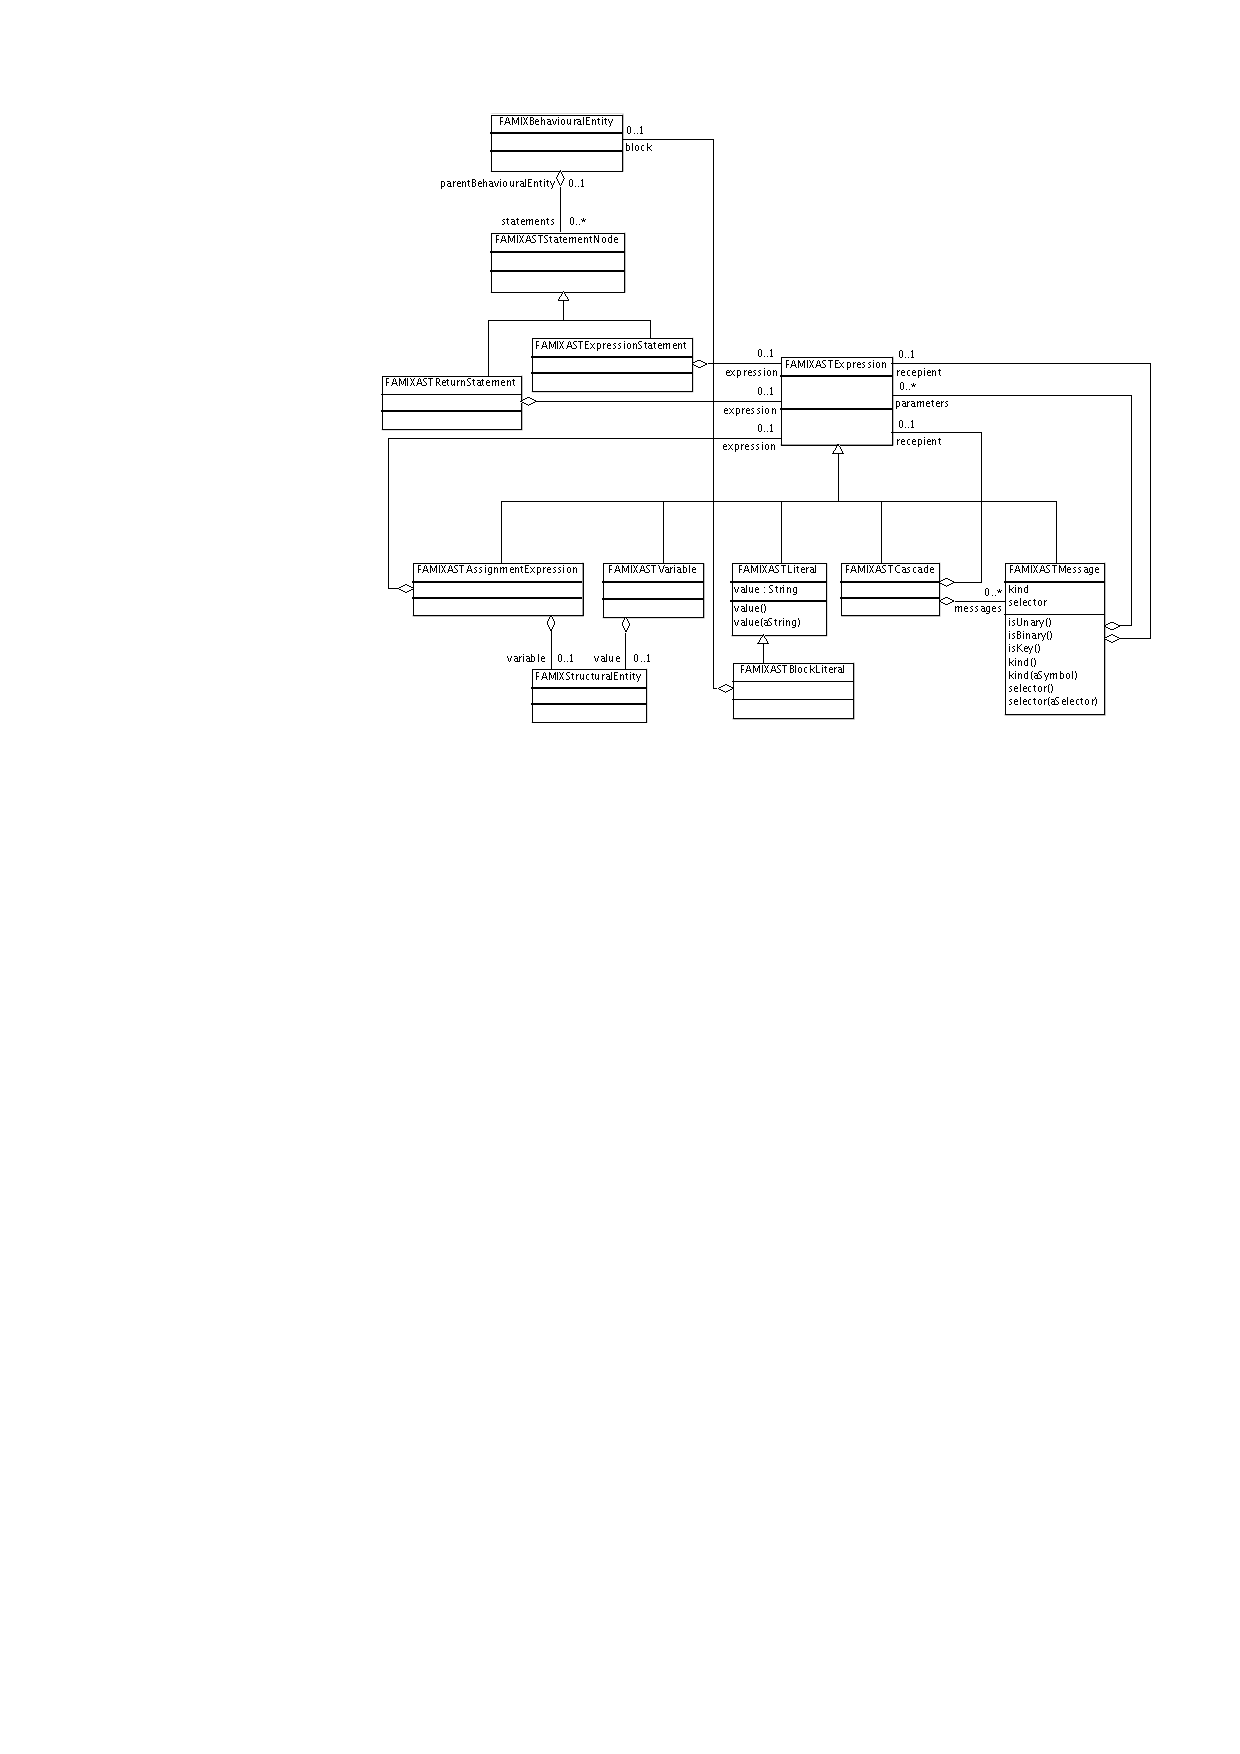
\includegraphics[width=0.95\textwidth]{SmalltalkASTClassDiagram}
  \caption{Діаграма FAST для смолтоку\label{smtFast}}
\end{figure}

Як видно з діаграми, в моделі FAST для смолтоку не тільки присутні ланки, які непритаманні для цієї мови, але й деякі деталі змодельовані не так, як це реалізовано в дереві браузера для рефакторингу.

Перш за все в цій моделі прирутня ланка FASTStatementBlock, яка являє собою набір речень. В C--подібних мовах ця структура обмежена фігурними дужками і є тілом методів, а також часто зустрічається як тіло інструкцій if, for, while та подібних. В смолтоці нічого подібного немає, але нам набагато легше мати зайвий прошарок, який можна оминути, чим потім робити великі зміни при абаптації C--подібних мов. Через цей нюанс в FASTBehaviouralEntity визначений метод \emph{statement}, який повертає всі речення з блоку речень. Таким чином ми можемо доступитись до речень бозпосередньо із сутності з поведінкою.

Також в смолтоці немає речень як таких. Абстрактне синтаксичне дерево браузера для рефакторингу містить просто визначення ланки повернення і ланки зі значенням на одному рівні з ланками методу та прагми. Так як смолток не є строго--типізованою мовою, то в ній не важливо будувати важкі ієрархії лише для того, щоб взірці різних класів могли знаходитись в одній колекції. Натомість середовище Moose передбачає щось в стилі сторогі типізації, адже прагми, які визначають властивості та зв'язки між ланками моделі, вказують тип цих зв'язків. Тим не менше ця концепція гарно вписується в синтакс смолтоку, і тому в нас присутні два типи речень: речення з виразом, та речення повернення з методу.

Щодо відмінності від моделі дерева у браузері для рефакторингу, то вона проявляється у структурі каскадного повідомлення. Оригінально каскадне повідомлення містило набір повідомлень, перше з яких містило отримувача, як показано на рис.~\ref{rbCascade}.
\begin{figure}[h]
        \vspace{\columnsep}
        \centering
        \begin{subfigure}[b]{0.45\textwidth}
                \centering
                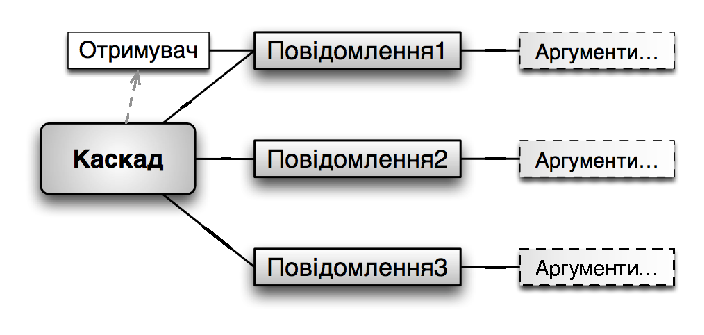
\includegraphics[width=\textwidth]{rbCascade}
                \caption{Браузер рефакторингу\label{rbCascade}}
        \end{subfigure}
        \hspace{0.05\textwidth}
        \begin{subfigure}[b]{0.45\textwidth}
                \centering
                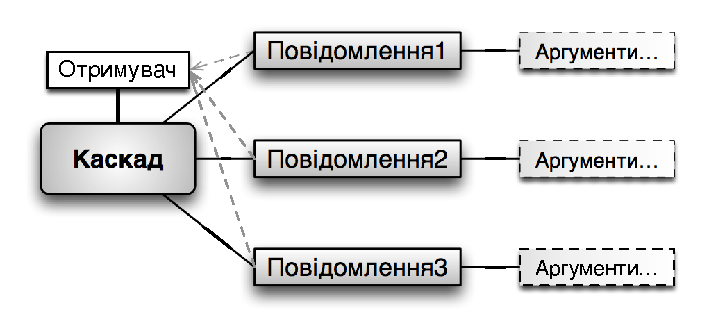
\includegraphics[width=\textwidth]{fastCascade}
                \caption{FAST\label{fastCascade}}
        \end{subfigure}
        \caption{Порівняння ралізацій моделі каскадного повідомлення}
\end{figure}
Штриховою лінією показано, що каскад має непрямий доступ до отримувача через перше повідомлення. Натомість у FAST отримувач безпосередньо зв'язаний з ланкою каскаду і всі повідомлення мають до нього непрямий доступ через каскад (рис.~\ref{fastCascade}). Перш за все це накладає одинакові умови на повідомлення --- всі вони не мають беспосереднього отримувача. Крім того така модель природніша для сприйняття, оскільки каскадне повідомлення якляє собою набір повідомлень, які надсилаються до одного і того ж об'єкту,

Можна також звернути увагу на особливість реалізації зворотнього зв'язку іменованої сутності. Як було згадано в основних ідеях FAST, ми хочемо мати зв'язок з батьківським ланками. Проблема полягає у „строгій типізації“ яку накладає платформа Moose. В іменованої сутності уже є зв'язок з батьківським виразом--іменованої сутності, але вона також може бути дочірньою ланкою виразу--присвоєння. Тому в іменованої сутності присутній ще один зворотній зв'язок з ланкою типу виразу--присвоєння. Таким чином, аналізуючи певну іменовану сутність ми можемо зразу сказати де вона використовується, а також перейти вверх по ієрархії ланок. 

\subsection{Спосіб створення моделі з вихідного коду}
Оригінально з метою створення FAST--моделі з вихідного коду, використовувався парсер браузеру для рефакторингу, який по замовчуванню присутній у Pharo. Згодом, коли для роботи з Java почав використовуватись PetitParser, генерацію моделі із Smalltalk було переведено на використання тієї ж технології. Результат роботи PetitParser для Smalltalk був ідентичний до результату парсера браузера для рефакторингу, але при використання одинакової технології в різних вітках цього проекту, дозволяє досягнути кращої якості.

\clearpage

\section{Мета--модель абстрактного дерева Java}

\subsection{Структура моделі}

\subsection{Спосіб створення моделі з вихідного коду}
Як і для смолтоку, модель абстрактного синтаксичного дерева Java потрібно будувати на вимогу, маючи в наявності вихідний код. Першим способом реалізації було розширення та викоритання програми VerveineJ. На даний момент саме вона використовується для побудови FAMIX моделей з вихідних файлів Java. Позитивними частинами цієї програми є використання нею JDT (Java Development Tools) бібліотеки середовища Eclipse, що значно полегшує генерацію абстрактного синтаксичного дерева джави з вихідного коду. Варто зауважити, що JDT генерує абстрактне синтаксичне дерево за специфікаціями Oracle, тому в подальшому його потрібно перетворити у FAST. Щодо поганих сторін такого підходу, то спочастку модель зберігається зовнішньою джава--програмою у ворматі MSE, а тоді вже читається середовищем Moose і перетворюється у FAMIX модель. Очевидно, що робота з проміжним форматом вже передбачає в собі слабке місце. Крім того використання зовнішньої джава програми означає залежність на JRE середовищі, наявності самої програми, а також функціональності бібліотек OSProces, які дозволяють викликати зовнішні скрипти з Фаро. Також розробка на двох різних платформах несе додаткове навантаження, так як приходиться доволі часто змінювати спосіб мислення щодо написання коду.

З другого боку на момент здійснення вибору вже існувала часткова реалізація парсера вихідного коду Java розроблена на основі PetitParser. Ця реалізація в собі включала повний лексикон та синтакс Java з тестами, а також частково реалізовиний парсер. Отже для використання цього парсера, щоб завантажувати FAST, передбачало ще й роботу над самим парсером. Тим не менше цей варіант був найкращим оскільки він використовував технології, які були застосовані в ланцюшжу інструментів FAST для роботи із Smalltalk. Таким чином використання PetitParser для всіх віток моделей FAST означає, що весь час призначений для покращення парсера не буде розпорошуватись на дікілька технологій, а буде зосереджений безпосередньо на одній. Аналогічно у цьому підході відсутні все негативні сторони VerveineJ.

\clearpage

\section{Symbol resolution}
При генераціїї абстрактного синтаксичного дерева з вихідного коду в якості листків графу ми можемо отримати \emph{іменовані сутності} або ж літерали. Іменована сутність несе лише інформацію про назву змінної чи класу і цього доволі мало для аналізу вихідного коду. Одинаковий ідентифікатор може зустрічатись в багатьох місцях програми, але відноситись до різних змінних. Для того, щоб визначити які сутності відносяться до тієї самої змінної будем використовувати \textbf{область визначення (scope)} змінної, а також мета--змінну яка буде знаходитись в цій області, і буде зв'язана з іменованими сутностями абстрактного синтаксичного дерева. Кожна область буде мати батьківську область визначення. Для методу це будуть змінні класу. Для класу - змінні пакету. Таким чином при пошуку змінної з певним ім'ям, якщо ми не знайдемо її в поточній області визначення, то зможемо продовжити пошуки в батьківській. Головне завдання о'бєкту області визначення:
\begin{enumerate}
\item знаходити мета--змінну за відповідною назвою.
\item додати мета--змінну з відповідною назвою
\item повернути сутність до якої ця область прив'язана. Наприклад: метод, клас, блок
\end{enumerate}

Перший пункт реалізується дуже легко. Для збереження інформації про взаємоз'язок назв і сутностей мета--змінних використовується просто словник в якому кожній назві відповідає певна змінна. На наступному прикладі можна деталініше розглянути, як працює даний метод:
\begin{lstlisting}[language=Smalltalk]
FAMIXScope>>resolve: name
	^ variables
		at: name
		ifAbsent: 
			[parent notNil 
				ifTrue: [parent resolve: name] 
				ifFalse: nil]
\end{lstlisting}
Все зводиться до отримання значення за ключем--назвою змінної. Якщо такого немає, то питаєм в батьківської області.

Другий пункт зводиться до заненнесення пари ключ--значення у словник. А третій пункт передбачає змінну взірця класу, яка буде вказувати на вланкика області, та отримувач і втановлювач змінної.

В якості мета--змінних використовуються сутності змінних визначені у FAMIX. Перш за все вони вже мають необхідну мета--інформацію, але крім того деякі моделі підчас генерації частково виконують резолюцію символів. Таким чином ми можемо використатви вже зроблену роботу.

В сутностей, які мають області визначення повинен бути метод для отримання цієї області. Пропонується використовувати ліниву ініцілізацію, так як деякі частини фамікс вже розв'язують проблему ідентифікації змінної. Таким чином у момент часу, коли комусь потрібно отримати область визначення, її вже можна буде наповнити деякими мета--змінними. Для прикладу розглянемо реалізацію такої лінивої ініціалізації для сутності методу моделі FAMIX:
\begin{lstlisting}[language=Smalltalk]
FAMIXMethod>>scope
	^ self privateState cacheAt: #fastScope ifAbsentPut: [
		| scope |
		scope := FASTScope newWithParent: self belongsTo scope.
		scope owner: self.
		self implicitVariables do: [:variable | scope add: variable].
		self parameters        do: [:variable | scope add: variable].
		self localVariables    do: [:variable | scope add: variable].
		scope]
\end{lstlisting}

Перш за все варто зауважити, що ми додаємо цей функціонал до класу зробленого кимсь іншим. Це ще одина позитивна сторона цього підходу, так як ми хочемо мати можливість застосовувати наш алгоритм до вже існуючих моделей, а не будувати все з нуля. Відповідно область визначення зберігається в приватному стані MooseEntity, але якщо ми хочемо отримати область вперше, то нам портібно перш за все її створити та ініціалізувати. Цей метод створює область визначення зразу з батьківською областю, яка отримується від батька поточної сутності. Далі сутність встановлює себе як власника області, і додає в неї всі неявні та локаліні змінні а також параметри. Таким чином, якщо на момент отримання області вже були якісь дані про змінні в даній сутності --- вони будуть скопійовані в область.

Щодо самого алгоритму резолюції символів, то він зводиться до відвідування моделі FAST та запитування поточної області про мета--змінну з даним ім'ям. Ось короткий приклад, як це зроблено в смолтоці:
\begin{lstlisting}[language=Smalltalk]
FASTResolutionVisitor>>acceptNamedEntityNode: aNamedEntityNode
	aNamedEntityNode famixVariable: (scope resolve: aNamedEntityNode name)
\end{lstlisting}

При отриманні відвідувачем ланки яка є іменованою сутністю, він їй в якості мета--змінної, присвоює результат виконання методу \lstinline$resolve:$ поточної області. Також можливі деякі модифікації, наприклад, створення „накопичуючої“ області, яка буде створювати нову змінну при її її відсутності. Таку область можна зробити найстаршою в ланцюжку батьківства. Таким чином в ній будуть накопичуватись наоголошені змінні. Аналогічно для скриптових мов програмування в яких немає явного оголошення змінних --- області повинні створювати змінні при першій їх появі.
\clearpage

\section{Метрики коду}
Маючи абстрактне синтаксичне дерево, дуже зручно обчислювати на ньому метрики. Так як наше синтаксичне дерево доволі абстрактне, то реалізувавши на ньому обчислення метрик коду, ми зможемо адаптувати алгоритм до різних мов програмування, моделей. 

Одною з найпростіших метрик є кількість \emph{речень} коду. Так як кожна сутність з поведінкою має в собі колекцію \emph{речень}, то весь алгоритм зводиться до обчислення розміру колекції, що вміє зробити сама колекція.

\subsection{Цикломатична складність}
Цикломатичною складністю вважається кількість можливи шляхів виконання коду. Наприклад, якщо програма не містить ніяких інстуркій галуження та циклів, то її можна пройти одним чином. Цикломатисна складність такої програми рівна 1. Якщо ж в програмі з'явиться одна інструкція галуження (\lstinline$if$), то її вже можна буде пройти двома способами. Це результує у цикломатичній складності 2. Аналогічне правило діє на циклах. 

Правило обчислення цикломатичної складності каже, що вона дорівнює кількості інструкцій галуження та циклів плюс 1. В такому випадку алгоритм буде еквівалентрий відвідуванню дерева. При цьому при отриманні ланки, яка збільшує цикломатичну складність --- збільшувати змінну взірця на 1. Цей алгоритм дозволяє враховувати навіть такі екзотичні випадки як інструкція циклу, що має альтернативний блок else у мові прогамування Python. Така інструкція збільшує цикломатичну складність програми на 2. Але ця особливість зводиться лише до визначення чергової дії відвідувача на отримання певної ланки абстрактного синтаксичного дерева.

Проблеми починаються у мовах з лямбда--функціями, блоками та замиканнями. Найкращим прикладом є, звичайно ж, Смолток. В цій мові прогамування інструкії циклів та галуження взагалі відсутні. На жаль в такому випадку важко сказати, чи конкретне повідомлення буде збільшувати цикломатичну складність, чи ні. Ми не знаємо якому саме об'єкту буде надіслано повідомлення, відповідно і не знаєм реалізацію. З цією метою будем використовувати метод аналогічний до того, що використовується в середовищі Moose. Визначим дві множини селекторів: галуження і циклів та додамо туди наперед відомі селектори, такі як \lstinline$ifTrue:ifFalse:$, \lstinline$whileTrue:$, \lstinline$detect:ifNone:$. Тоді при визначенні чи повідомлення збільшує цикломатичну складність будем перевіряти, чи воно присутнє в тій чи іншій колекції. Варто звернути додаткову увагу на використання двох колекцій, а не одної. Селектор \lstinline$detect:ifNone:$ повинен бути в обок колекціях, так як його реалізація включає в себе як цикл так і галуження. Тому при при визначенні цикломатичної складності, він буде виявлений в обох колекціях, і тому збільшить складність на 2 \cite{cyclocomplexity-moose}.

\subsubsection{Удосконалення алгоритму відвідувача}
Як вже було описано вище --- алгоритм зводиться до відвідування ланок дерева, і при опрацюванні тої чи іншої ланки додавання збільшення загальної цикломатичної складності в залежності від певних умов, скажімо типу селектора. Але це означає, що для кожної особливої ланки нам потрібно буде перевизначати поведінку відвідувача. Натомість цю логіку можна перенести всередину самого об'єкту. Нехай будь яка ланка, яка відповідає певному вихідному коду буде знати свій внесок у цикломатичну складність. У FAMIX такій ланці відповідає клас FAMIXSourcedEntity. В ньому ми можемо визначити метод \emph{cyclomaticComplexityContribution}, який буде повертати 0. Тоді для кожного класу, який буде відображати ланку, що впливає на цикломатично складність, цей метод буде перевизначатись. Наприклад для інструкцій if, for, while в мові джава цей метод буде повертати 1. Для інструкції for ... else в мові Python, цей метод буде повертати 2, так як вона об'єднує в собі цикл і галуження. Для повідомлень у смолтоці цей метод буде обчислювати внесок складності динамічно, адже він буде залежати від селектора повідоблення. Ще одним плюсом цього методу є можливість кешування обчислених даних в самій ланці, таким чином їх не треба буде перераховувати всі наступні рази. Також внесок цикломатичної складності можна зробити властивістю ланки, що дозволить переглядати цю інформацію в панелі середовища Moose.

\clearpage

\addcontentsline{toc}{section}{Література}
\begin{thebibliography}{9}

\bibitem{moose}Tudor Girba, \emph{The Moose Book} [Електронний ресурс],
    2011. Режим доступу:
    \url{http://www.themoosebook.org/book/table-of-contents}

\bibitem{mse-famix}S.Ducasse, J.Laval, N.Anquetil, A.Cavalcante-Hora, U.Bhatti, \emph{MSE and FAMIX 3.0: an Interexchange Format and Source Code Model Family} [Електронний ресурс], 2011. Режим доступу:
    \url{http://rmod.lille.inria.fr/archives/reports/Duca11c-Cutter-deliverable22-MSE-FAMIX30.pdf}
    
\bibitem{astm-spec}Object Management Group, Inc., \emph{Abstract Syntax Tree Metamodel (ASTM) Specification} [Електронний ресурс], 2008. Режим доступу:
    \url{http://www.omg.org/spec/ASTM/1.0/Beta1/PDF}

\bibitem{cyclocomplexity-moose}Adrian Kuhn, \emph{Cyclomatic Complexity in Languages with Closures} [Електронний ресурс], 2009. Режим доступу:
    \url{http://www.iam.unibe.ch/~akuhn/blog/2009/cyclomatic-complexity-in-languages-with-closures/}

\bibitem{meet-grammars}Yuriy Tymchuk, \emph{Meet the grammars} [Електронний ресурс], 2013. Режим доступу:
    \url{http://uko-on-code.blogspot.fr/2013/02/grammars-complexity-comparison.html}

\end{thebibliography}

\end{document}
